\documentclass[13pt]{beamer}

\usepackage{Handle}
\usepackage[export]{adjustbox}

\newcommand{\Title}{Plasma }
\newcommand{\Subtitle}{MHD}
\newcommand{\Institute}{Motilal Nehru National Institute of Technology}
\newcommand{\InstituteAddress}{Prayagraj, U.P.}
\newcommand{\SubmittedBy}{Saurabh Gupta}
\newcommand{\SubmittedTo}{Dr. Supriya Yadav }
\newcommand{\ImageUrl}{Images/plasma.jpg}




\subject{DAA}

\small
\date{\today}




\begin{document}
	\begin{frame}[noframenumbering,plain,t]

		\begin{tikzpicture}[remember picture, overlay]
			\node[opacity = 0.8] at (current page.center)
			{
				
\includegraphics[height = 1.5\paperwidth]{Images/bg4.png}
			};
		\end{tikzpicture}

		\MakeTitle

	\end{frame}


	\begin{frame}{Outline }
		\begin{tikzpicture}[remember picture, overlay]
			\node[opacity = 0.2] at (current page.center)
			{
				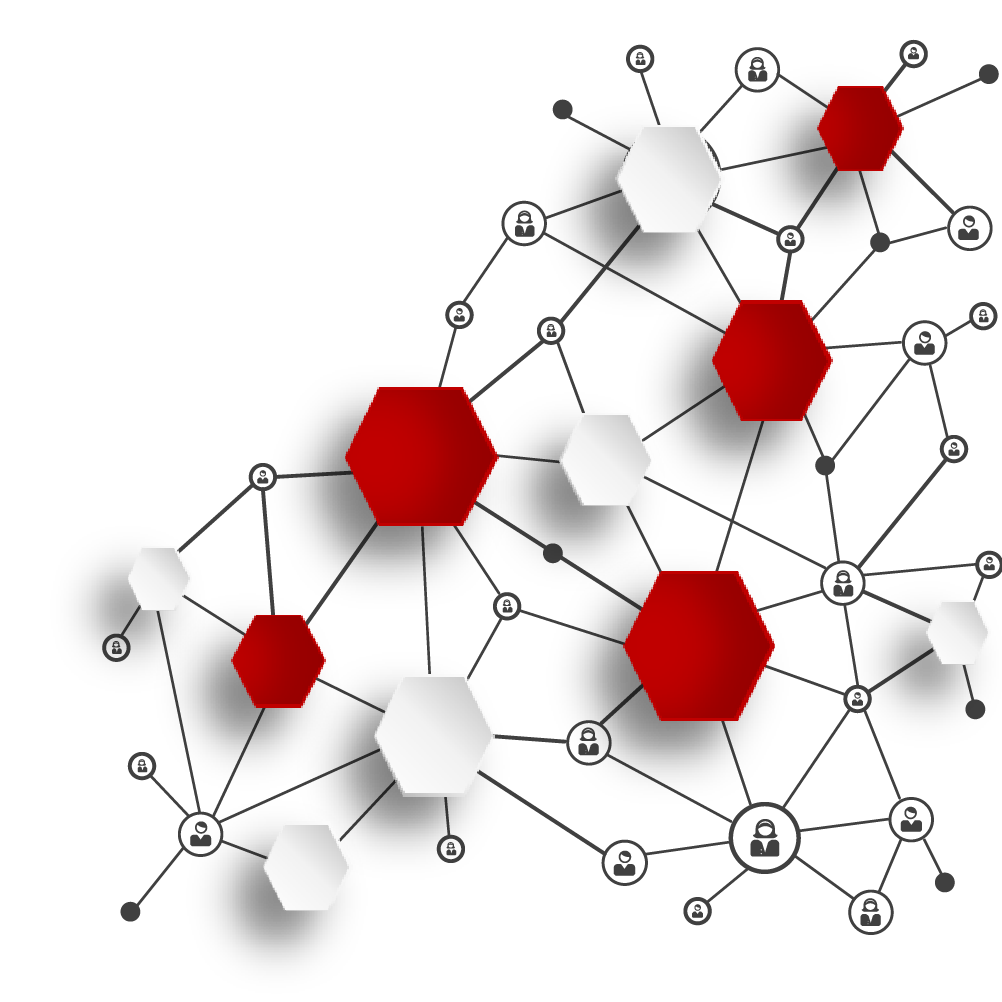
\includegraphics[height = 0.75\paperwidth]{Images/bg3.png}
			};
		\end{tikzpicture}

		\normalsize
		\tableofcontents
	\end{frame}


	\section{Introduction}
	   \setbeamercolor{section in head/foot}{bg=arsenic,fg=white}
	\setbeamercolor{frametitle}{bg=arsenic,fg=white}
	\setbeamercolor{author in head/foot}{bg=arsenic,fg=white}

	\begin{frame}[t]{What is Plasma ?}
       Plasma is often referred to as the fourth state of matter, distinct from solid, liquid, and gas. It is an \textbf{ionized gas} composed of positively charged ions and free electrons.

			\begin{bee}[Only gas ?]{white}{arsenic}
				No, Plasma is any matter that’s ionized, and for solids such as a metal that usually means very high temperatures.
			\end{bee}

		\begin{figure}

			\href{https://www.collegenp.com/uploads/2023/10/Plasma-The-Fourth-State-of-Matter-Explained.jpg}{
				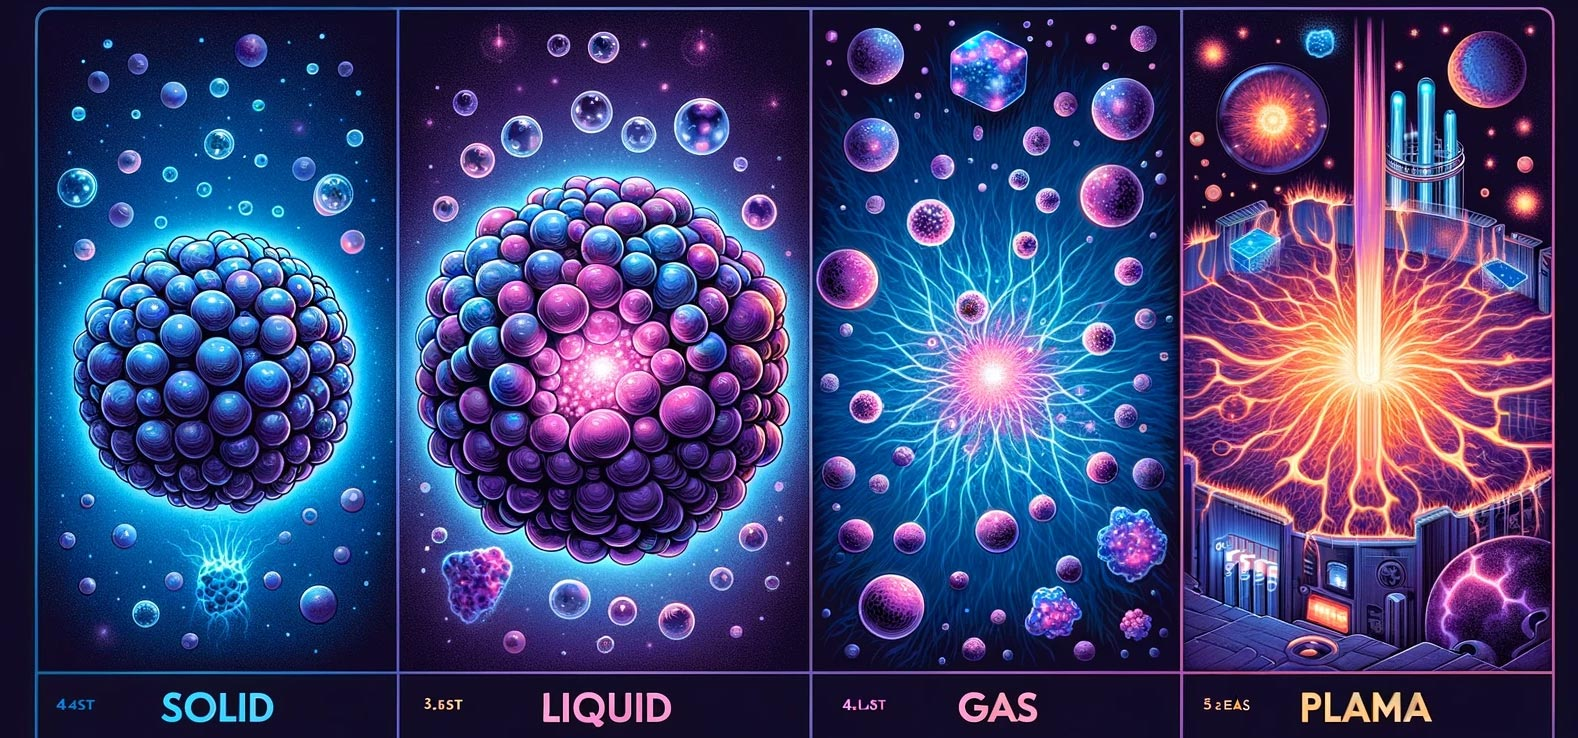
\includegraphics[height =0.16\textwidth]{Images/state of matter.jpg}
			}
		\end{figure}



	\end{frame}


	\section{Formation}

	\begin{frame}[t]{Formation of Plasma}
		\begin{itemize}
			\item Plasma is often formed through the process of {\color{magenta}ionization}.
		\item	At high temperatures, atoms gain enough energy to overcome the electrostatic forces holding electrons in their orbits around the nucleus.

		\item 	As a result, electrons are stripped away from the atoms, leading to the formation of positively charged ions and free electrons.
		\item {\color{red} High temperatures, electric discharges, or strong electromagnetic fields} can cause ionization.



		\end{itemize}
%
%
%		\begin{columns}
%			\column{0.5\textwidth}
%			\begin{bee}[Undirected Graph,width = 6cm]{black}{aqua}
%				A graph in which edges do not have any direction.
%			\end{bee}
%			\column{0.55\textwidth}
%			\begin{Rbee}[Directed Graph,width = 6cm]{arsenic}{aqua}
%				A graph in which edge has direction.
%			\end{Rbee}
%		\end{columns}
%		\begin{figure}
%			\centering
%			\href{https://media.geeksforgeeks.org/wp-content/uploads/20200630114438/directed.jpg}{
%				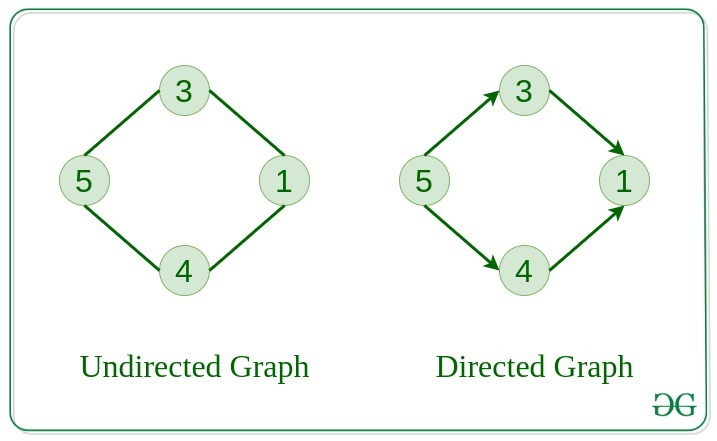
\includegraphics[height =0.37\paperheight]{Images/directed.png}
%			}
%		\end{figure}

%
%		\begin{bee}[Complete Graph,width = 8cm]{white}{deepmagenta}
%			A graph in which every pair of distinct nodes is connected by an edge
%		\end{bee}
%
%		\begin{Rbee}[Forest,width = 0.9\paperwidth]{white}{arsenic}
%			A collection of trees or disjoint tree-like structures within a graph
%		\end{Rbee}
%		\begin{bee}[Tree,width = 0.9\paperwidth]{white}{blue}
%			A special case of an acyclic graph in which there is a single root node, and every other node is connected by exactly one edge.
%		\end{bee}
%

	\begin{figure}
	\centering
		\href{https://www.collegenp.com/uploads/2023/10/Plasma-The-Fourth-State-of-Matter-Explained.jpg}{
	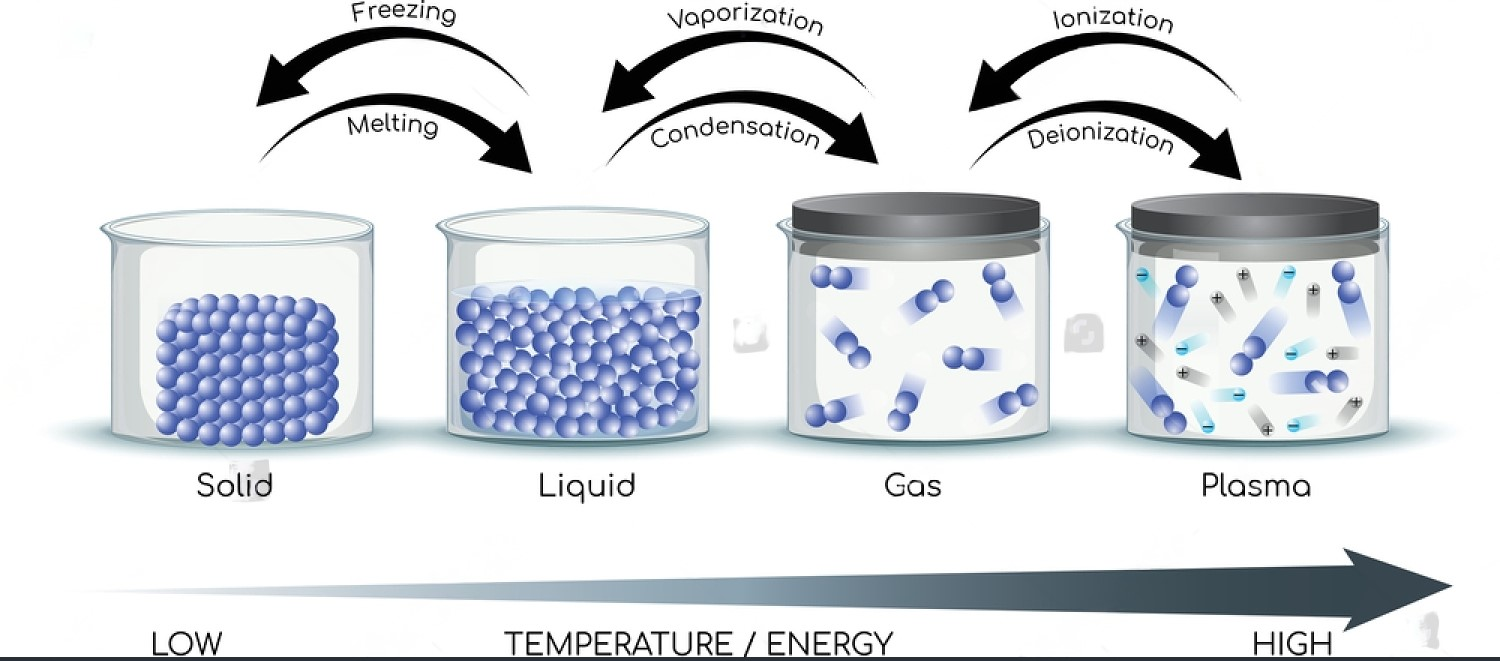
\includegraphics[width = 5.5cm]{Images/formation.jpeg}}
\end{figure}



	\end{frame}

     \section{Properties of Plasma}
	\begin{frame}[t,allowframebreaks]{Behavior/Properties of Plasma}

		\begin{itemize}
			\item 	\textbf{Electric Conductivity: }One of the defining features of plasma is its excellent electrical conductivity.
			The presence of free electrons allows for the transmission of electric currents.

			\item \textbf{Magnetic Interactions:} Charged particles in plasma respond to magnetic fields. The behavior of plasma is influenced by the interactions between charged particles and magnetic fields, leading to phenomena like magnetic confinement in fusion devices.


		\item \textbf{High Energy:} Plasma has high energy levels compared to other states of matter, making it capable of unique interactions and reactions.

			\item \textbf{Light Emission:} When electrons recombine with ions, they release energy in the form of light. This phenomenon is observable in various types of plasmas, such as neon lights and fluorescent tubes.

			\item \textbf{Fluid-Like Behavior: }Plasma exhibits fluid-like behavior, capable of flowing and taking on different shapes in response to external forces.


		\end{itemize}


	\begin{figure}
	\centering
	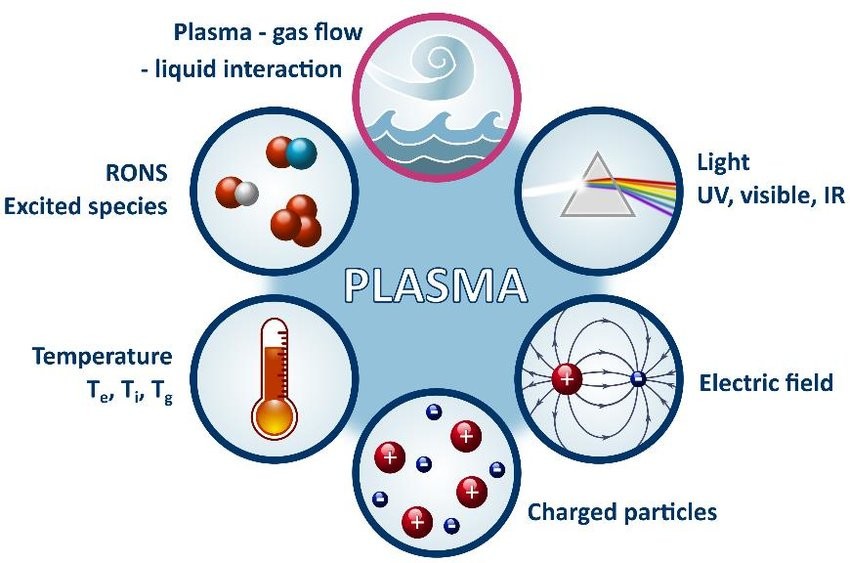
\includegraphics[width = \textwidth]{Images/props.png}
\end{figure}

	\end{frame}

\section{Application of Plasma}
\begin{frame}[t,allowframebreaks]{Applications of Plasma}
\begin{itemize}
		\item  \textbf{Plasma display : }
		\begin{figure}
			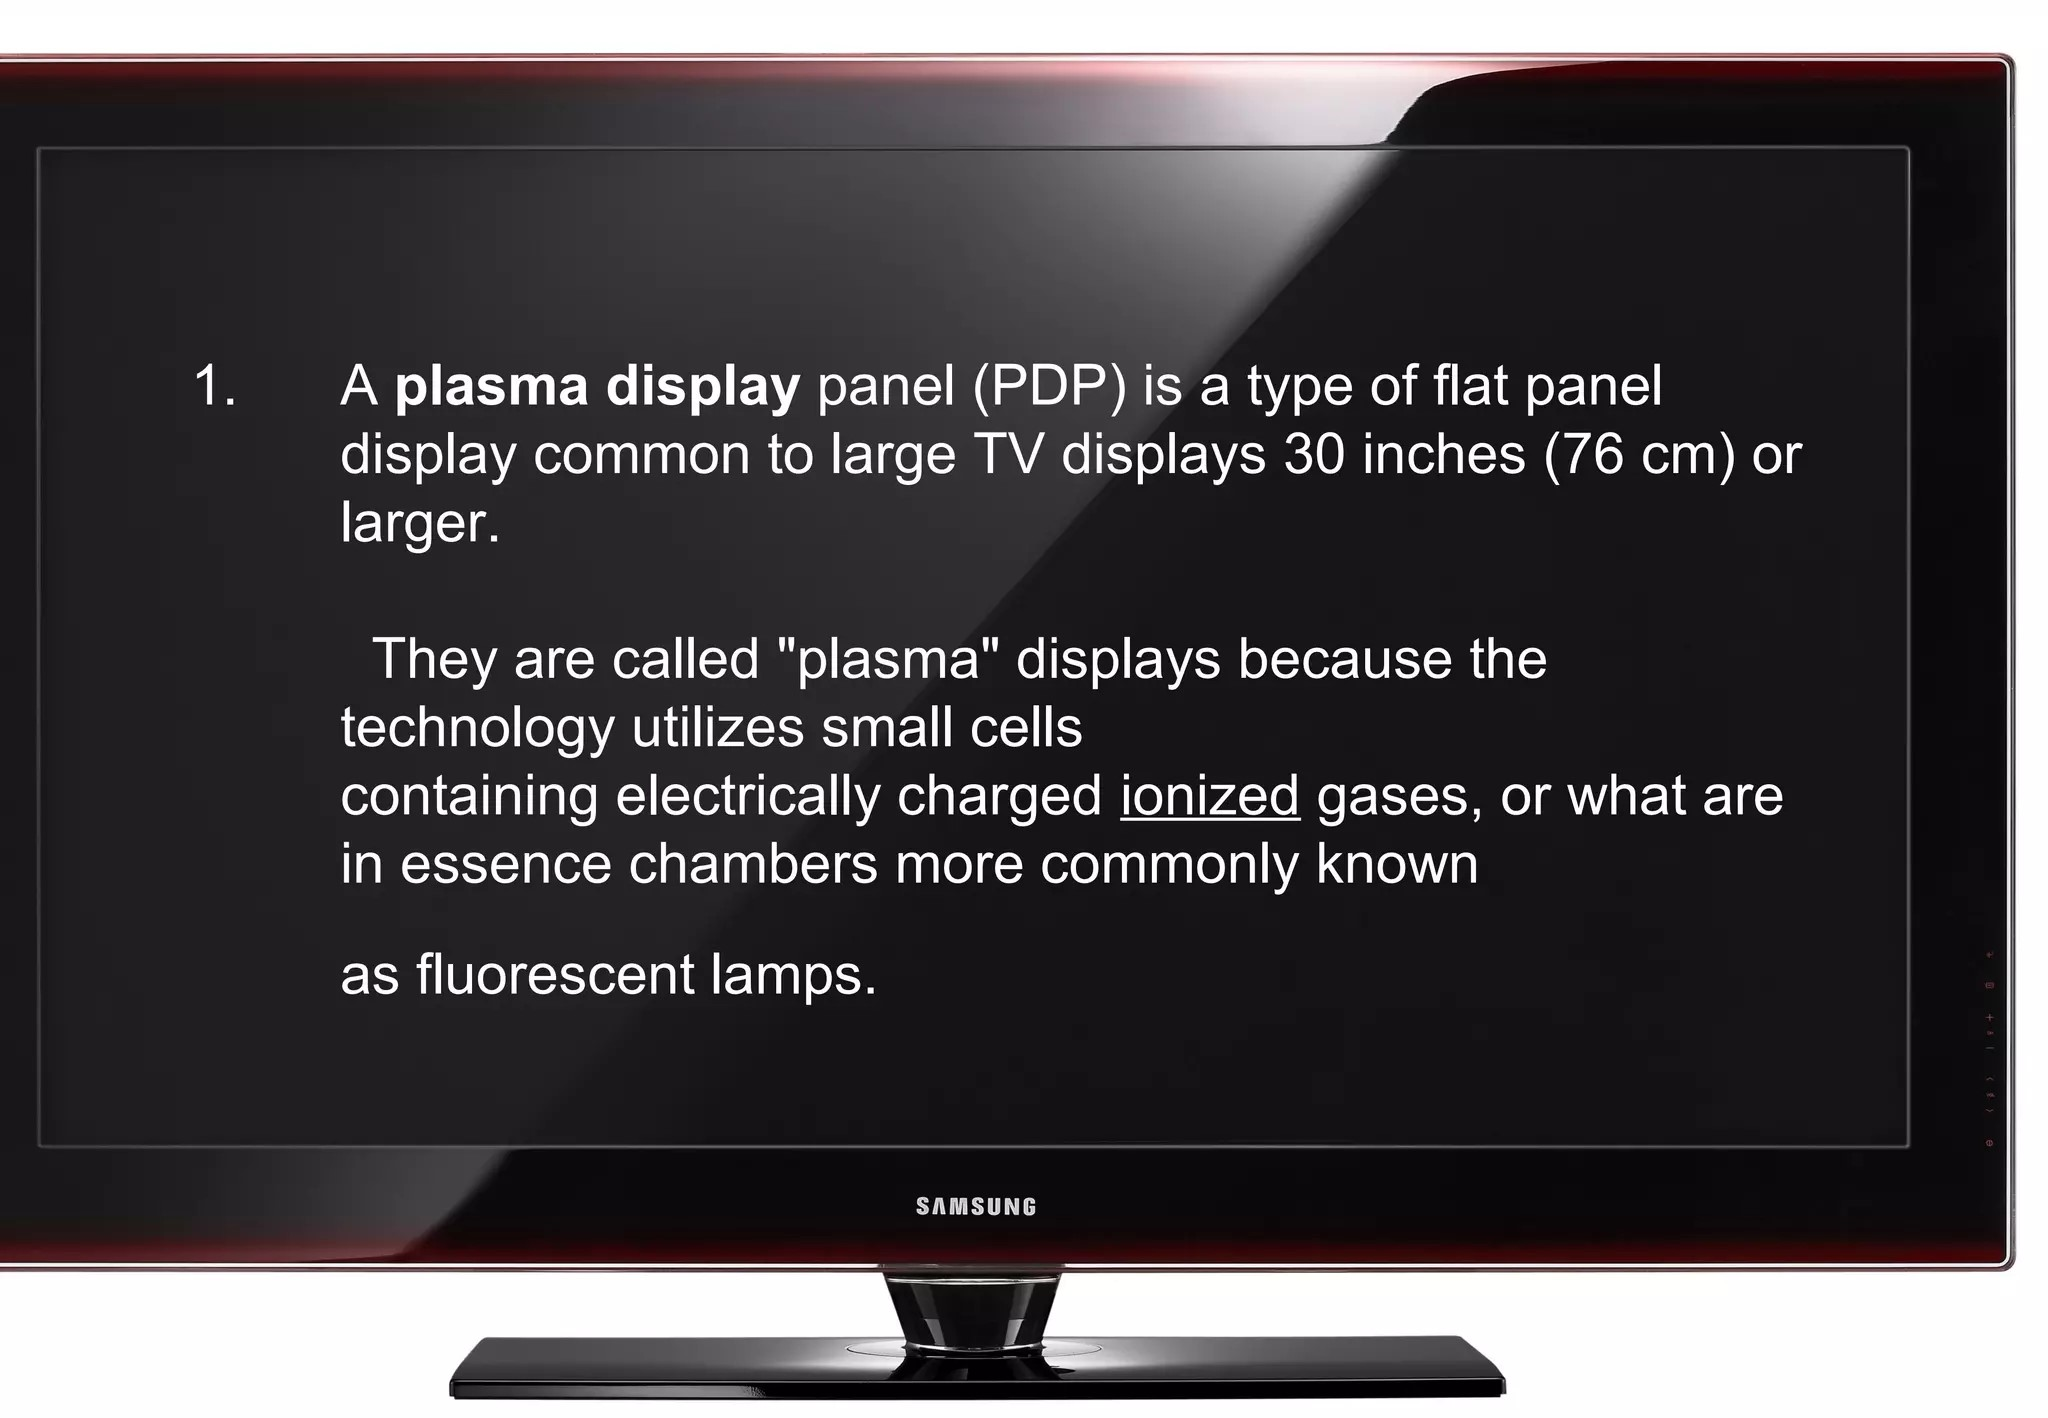
\includegraphics[height= 0.5\textwidth]{Images/apps (1).jpg}
		\end{figure}


		\item  \textbf{Welding Torch : }
		\begin{figure}
			\centering
			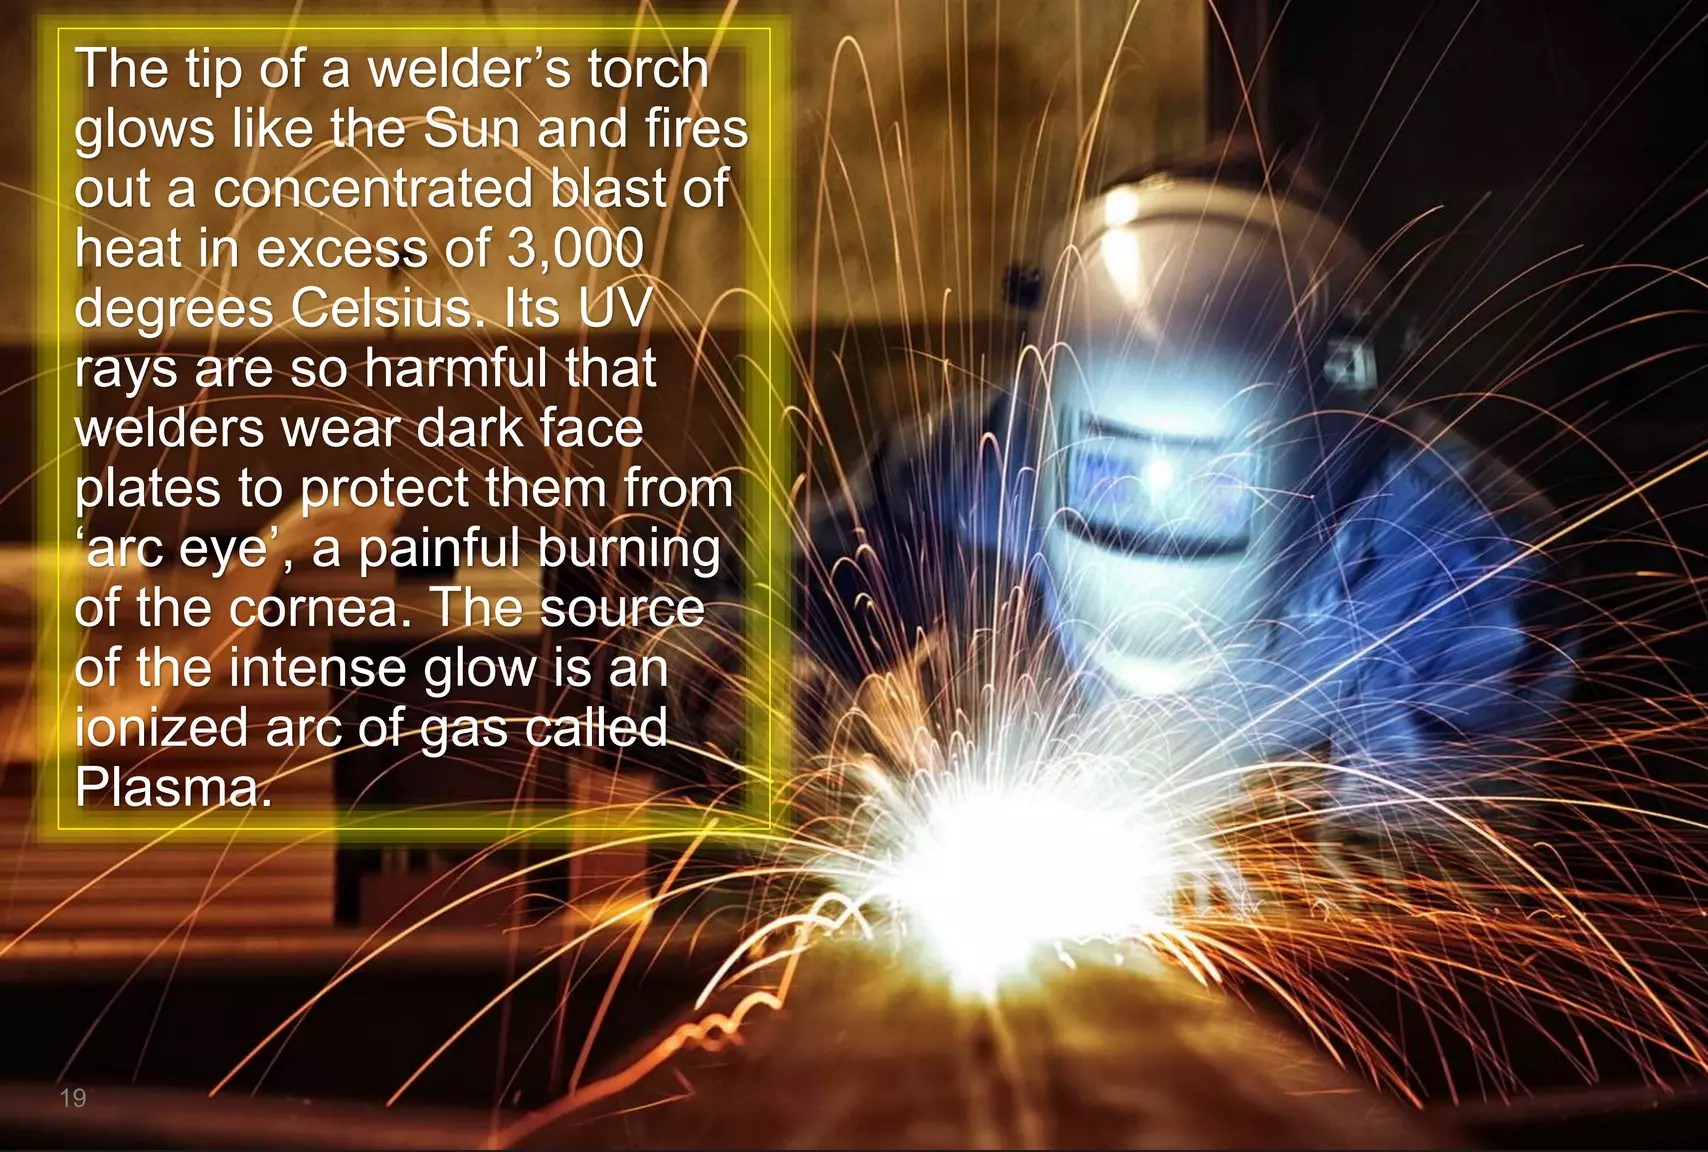
\includegraphics[height=0.5\textwidth]{Images/apps (3).jpg}
		\end{figure}

\end{itemize}


	 \textbf{Space Exploration:} \\
		Understanding and harnessing plasma is essential for space propulsion systems, as ion thrusters utilize electrically charged particles for propulsion.
		\begin{wrapfigure}{r}{0.5\textwidth}
			\centering
			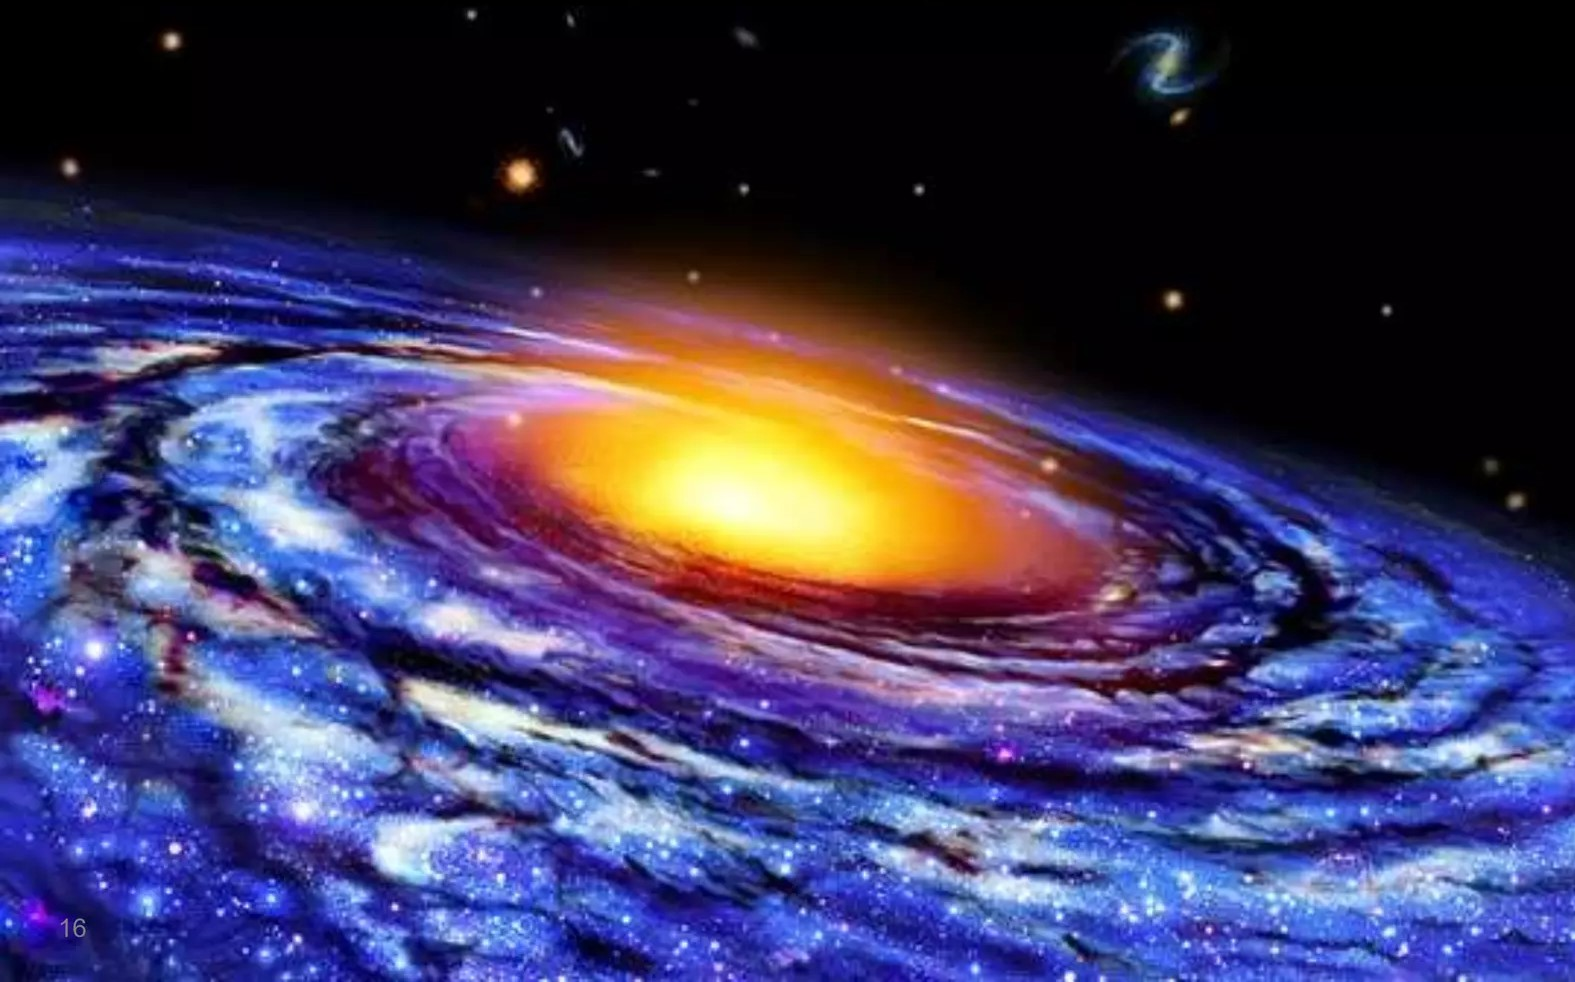
\includegraphics[height=0.3 \textwidth]{Images/apps (2).jpg}
		\end{wrapfigure}
		\\
		  Plasma is present everywhere in space, constituting a significant portion of the universe like stars and Galaxies.
		Studying astrophysical plasmas helps us understand celestial phenomena.








		 \begin{columns}

 	\column{0.45\textwidth}

\begin{figure}
	\centering
	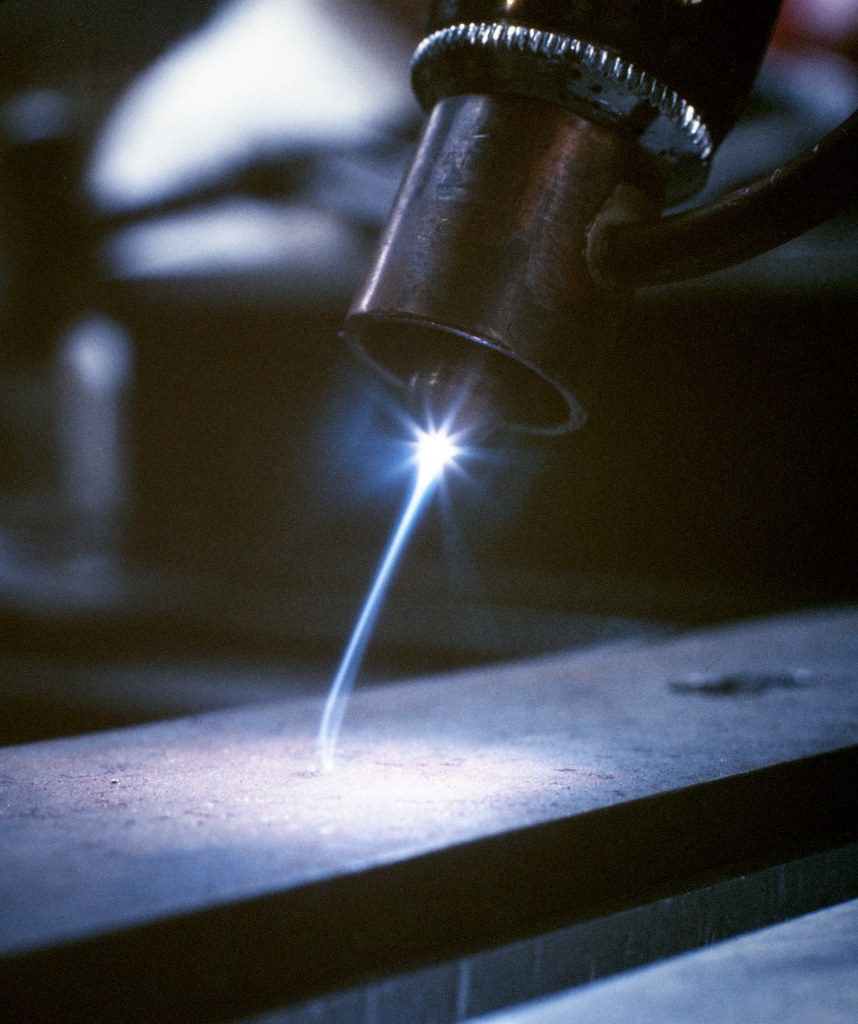
\includegraphics[width = \textwidth]{Images/application.jpg}
\end{figure}

		 	\column{0.65\textwidth}
		 	\begin{itemize}
		 	\item 	\textbf{Medical Applications:}\\
		 	Plasma plays a role in medical treatments, such as plasma donation for transfusions and plasma-based therapies.

		 	\item 	\textbf{	Material Processing:}\\
		 	Plasma cutting is used for precise cutting of metals, and plasma-based technologies contribute to surface modification and material synthesis.
		 \end{itemize}


		\end{columns}






\end{frame}

\section{MHD and Plasma}
\begin{frame}[t,allowframebreaks]{MHD and Plasma}
	The study of plasma in the context of magnetohydrodynamics (MHD) involves understanding the behavior of ionized gases (plasma) in the presence of magnetic fields. Let's explore the detailed theory and concepts related to plasma and magnetohydrodynamics: \\
	\vspace{0.5cm}
	\begin{itemize}
		\subsection{Basic MHD Equations}
		\item \textbf{Basic MHD Equations:} The fundamental MHD equations describe the behavior of plasma in the presence of magnetic fields. These equations include:
		\begin{itemize}
			\vspace{0.2cm}
			\item \textbf{Continuity Equation:} Describes the conservation of mass in a fluid, including a term for the movement of charged particles in the plasma.

		\item	\textbf{Momentum Equation:} Combines fluid dynamics with electromagnetic forces, accounting for the interaction between the fluid motion and magnetic fields.

		\item	\textbf{	Induction Equation:}Describes the evolution of magnetic fields in the plasma, taking into account the motion of the conducting fluid.

		\item	\textbf{	Energy Equation:}Incorporates energy transfer mechanisms, including heating and cooling processes, in the presence of magnetic fields.

		\end{itemize}

		\subsection{Magnetic Confinement}
		\item	\textbf{Magnetic Confinement:} MHD plays a central role in the design and operation of magnetic confinement devices, where the goal is to confine and \framebreak control the hot plasma. \\
		By using strong magnetic fields, MHD helps prevent the
		 plasma from dissipating and losing heat, allowing it to reach the required conditions for nuclear fusion. \\
		Examples of magnetic confinement systems include
				\href{https://en.wikipedia.org/wiki/Tokamak}{\underline{tokamaks}}, which use toroidal magnetic fields, and \href{https://en.wikipedia.org/wiki/Stellarator}{\underline{stellarators}}, which have more complex, three-dimensional magnetic field configurations.


 \begin{columns}

	\column{0.65\textwidth}



	\href{https://www.psfc.mit.edu/files/psfc/styles/researchtopicimage/public/imce/research/topics/alcator_c-mod_1000x450.jpg?itok=gNPMdhVj}{
		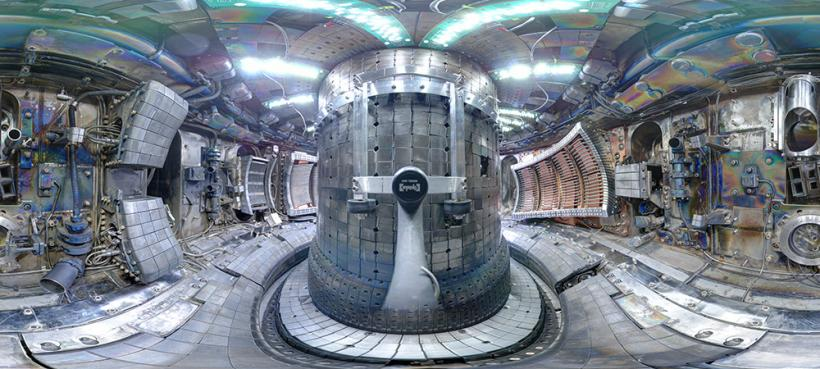
\includegraphics[height =0.4\textwidth]{Images/tokamaks.jpg}
	}

	\column{0.45\textwidth}

	\href{https://pbs.twimg.com/media/Drv63yvX0AAdsFF.jpg:large}{
		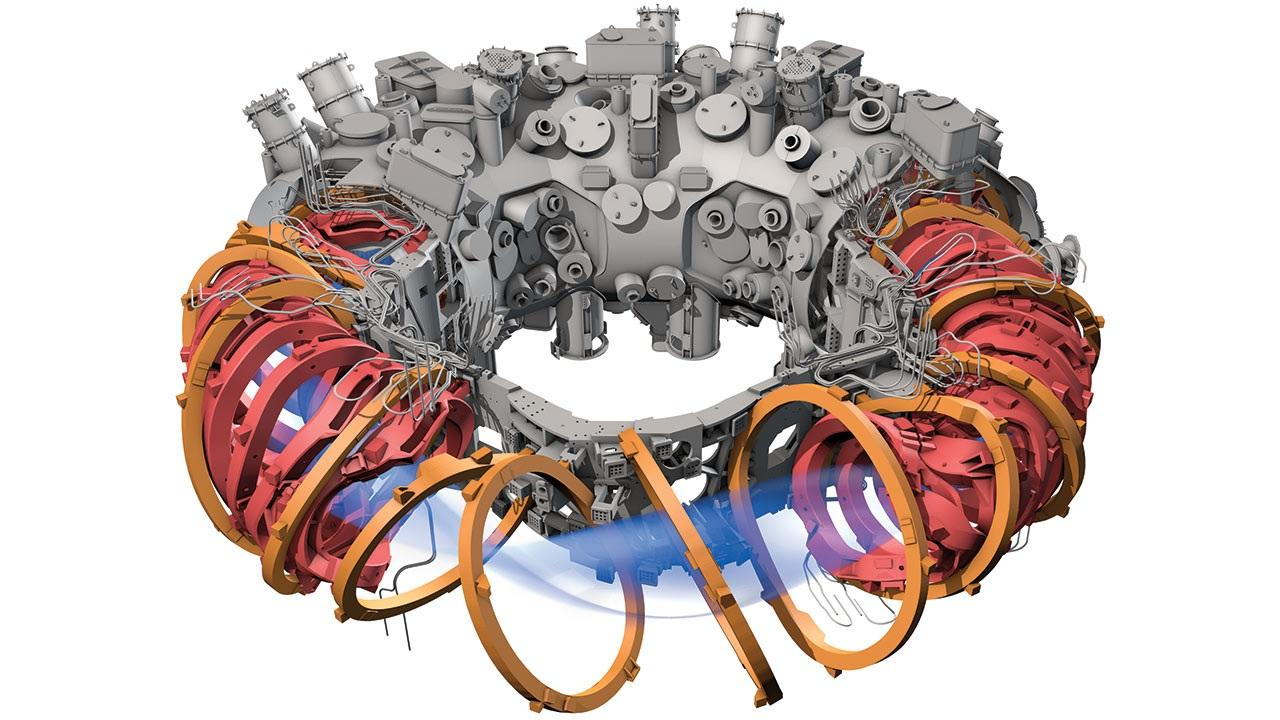
\includegraphics[height =0.5\textwidth]{Images/staller.jpg}
	}

\end{columns}

		\subsection{Plasma as a Conductive Medium}
	\item	\textbf{	Plasma as a Conductive Medium:} In MHD, plasma is considered a conductive medium due to the presence of charged particles (ions and electrons). The behavior of the plasma is influenced by its electrical conductivity, which is much higher than that of non-ionized gases.

	\subsection{Nuclear Fusion Research}
	\item	\textbf{	Nuclear Fusion Research:} One of the primary applications of MHD is in the field of nuclear fusion. In the quest for controlled nuclear fusion, MHD principles are crucial for maintaining and controlling the hot, ionized gas (plasma) at the high temperatures and pressures required for fusion reactions.

	 Devices like tokamaks and stellarators use magnetic fields to confine and stabilize the plasma,\framebreak preventing it from touching the walls of the containment vessel and facilitating controlled fusion reactions.
		\subsection{Astrophysical Applications}
		\item	\textbf{Astrophysical Applications:}
		\begin{itemize}
			\item	\textbf{Solar Wind:}MHD principles are applied to understand the  behavior of the solar wind, which consists of charged particles streaming from the Sun.

			\item	\textbf{	Stellar Magnetic Fields:}MHD is used to model the generation and evolution of magnetic fields in stars, influencing their structure and activity.
		\end{itemize}
	\subsection{Space Propulsion}
	\item	\textbf{	Space Propulsion:} MHD principles are applied in the development of electric propulsion systems for space exploration.
	\framebreak
	Ion thrusters, which use electrically charged particles (often xenon ions) as propellant, leverage MHD concepts to ionize and accelerate the propellant using magnetic and electric fields. This technology provides efficient and long-duration thrust compared to traditional chemical rockets.\\
\centering
\href{https://www.mdpi.com/applsci/applsci-13-05600/article_deploy/html/images/applsci-13-05600-g001.png}{
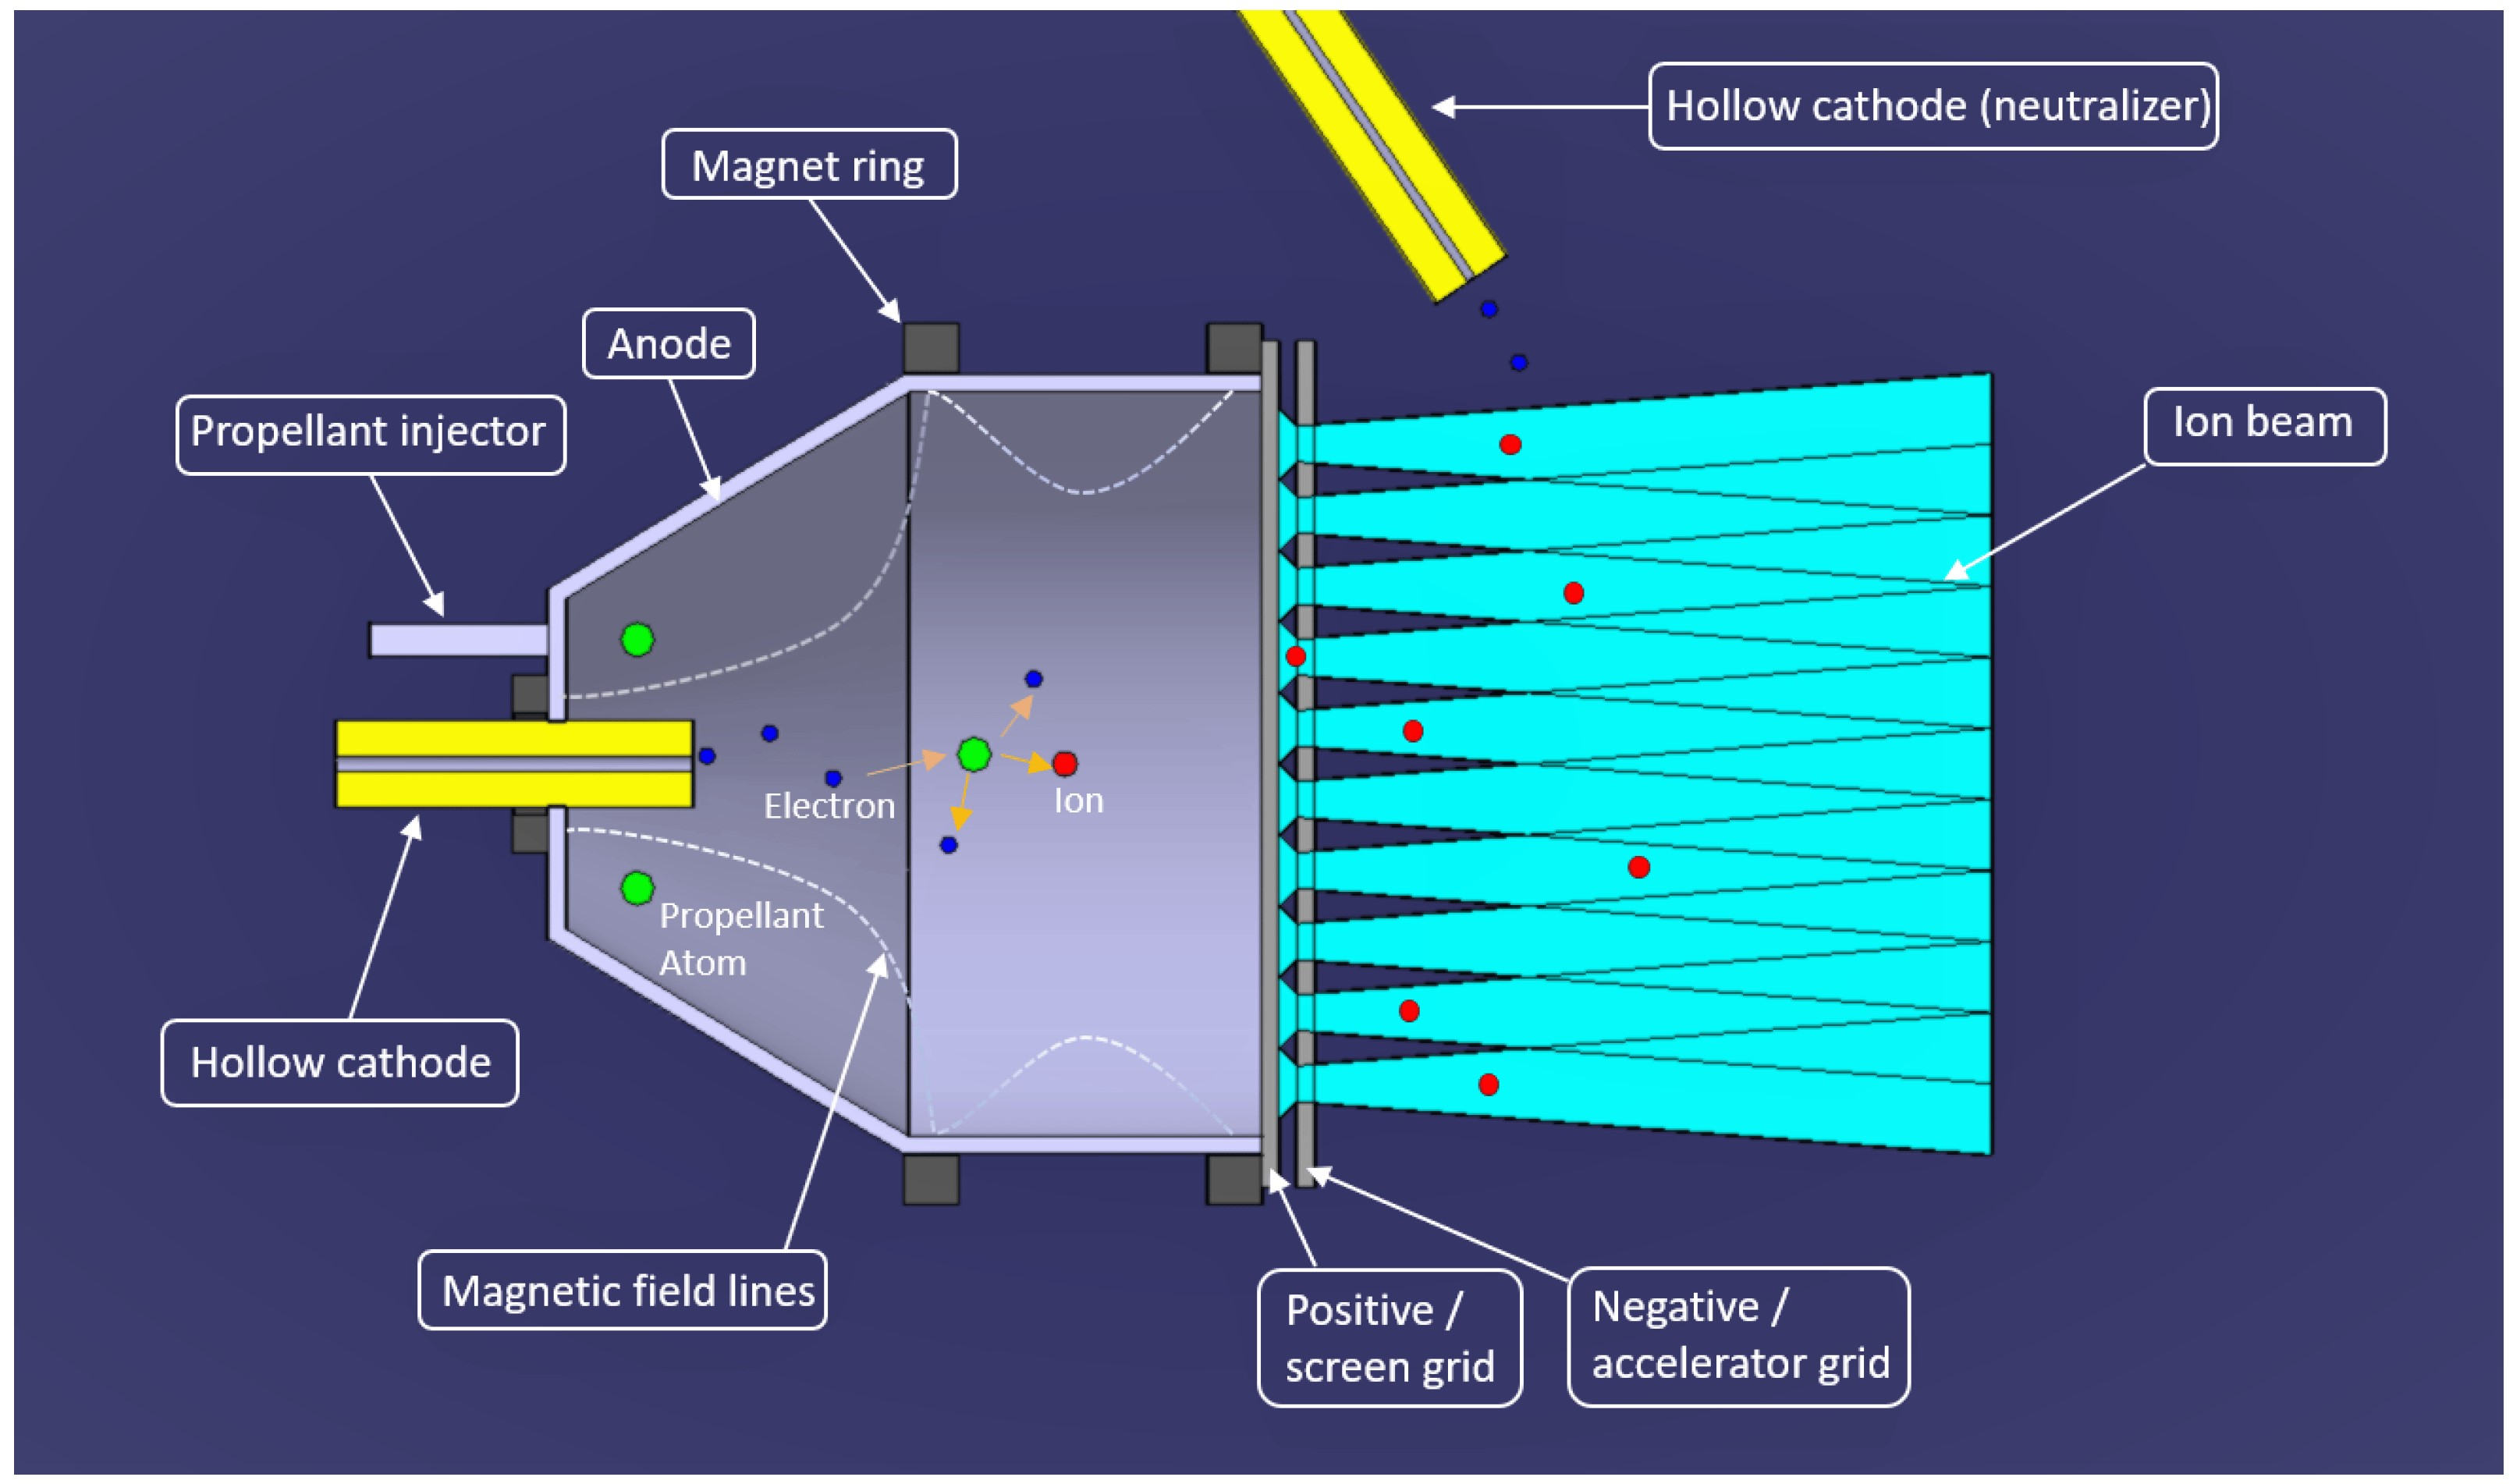
\includegraphics[width=0.8\textheight]{Images/ion thustors.jpg}
}


	\end{itemize}
\end{frame}


\section{Conclusion}
\begin{frame}[t]{Conclusion}

\begin{itemize}
	\item Magnetohydrodynamics provides a powerful framework for understanding and manipulating plasmas, especially in the context of nuclear fusion research and astrophysical phenomena.
	\item 	The combination of fluid dynamics and electromagnetic principles allows scientists and engineers to model and control complex plasma behaviors, with the ultimate goal of harnessing fusion energy for practical use.
	\item 	Ongoing research in MHD continues to advance our understanding of plasmas and improve the prospects for controlled fusion as a sustainable energy source.

\end{itemize}



\end{frame}

\begin{frame}

	\begin{figure}

		
\includegraphics[width = \textwidth]{Images/thanks.png}
	\end{figure}

%	\begin{figure}
%		\centering
%		
\includegraphics[width = 3cm]{Images/smile-removebg-preview.png}
%	\end{figure}

\end{frame}
\end{document}